\begin{figure}
	\centering%
	\setlength{\imagewidth}{140mm}%
	\setlength{\imageheight}{0.75\imagewidth}%
	\definecolor{colorEdS}{HTML}{64CF36}%
	\colorlet{colorEdSPoint}{black}%colorEdS!75!black}
	\definecolor{colorSphere}{HTML}{CD6E33}%
	\definecolor{colorCercle}{rgb}{0.049, 0.363, 1}%
	\DTLsetseparator{,}%
	\DTLloaddb[noheader,keys={x,y}]{dbspinepttng}{figures/data/EdS_propre_courbe/spine_point_tangent.dat}%
	\DTLloaddb[noheader,keys={x,y}]{dbcirclectrpt}{figures/data/EdS_propre_courbe/circle_center_point.dat}%
	\DTLloaddb[noheader,keys={x,y}]{dbenvelope}{figures/data/EdS_propre_courbe/envelope_data.dat}%
	\begin{tikzpicture}[
		x = \imagewidth,
		y = \imageheight,
		point/.style = {circle, scale=0.27, fill=black},
		vector/.style = {-latex', thick},
		label/.style = {inner sep=2pt},
		txt/.style = {font=\small},
	]
		\begin{scope}
			\clip (0.05,0.13) rectangle (0.95,0.97);	
			%
			\node[anchor=south west, inner sep=0] at (0,0) {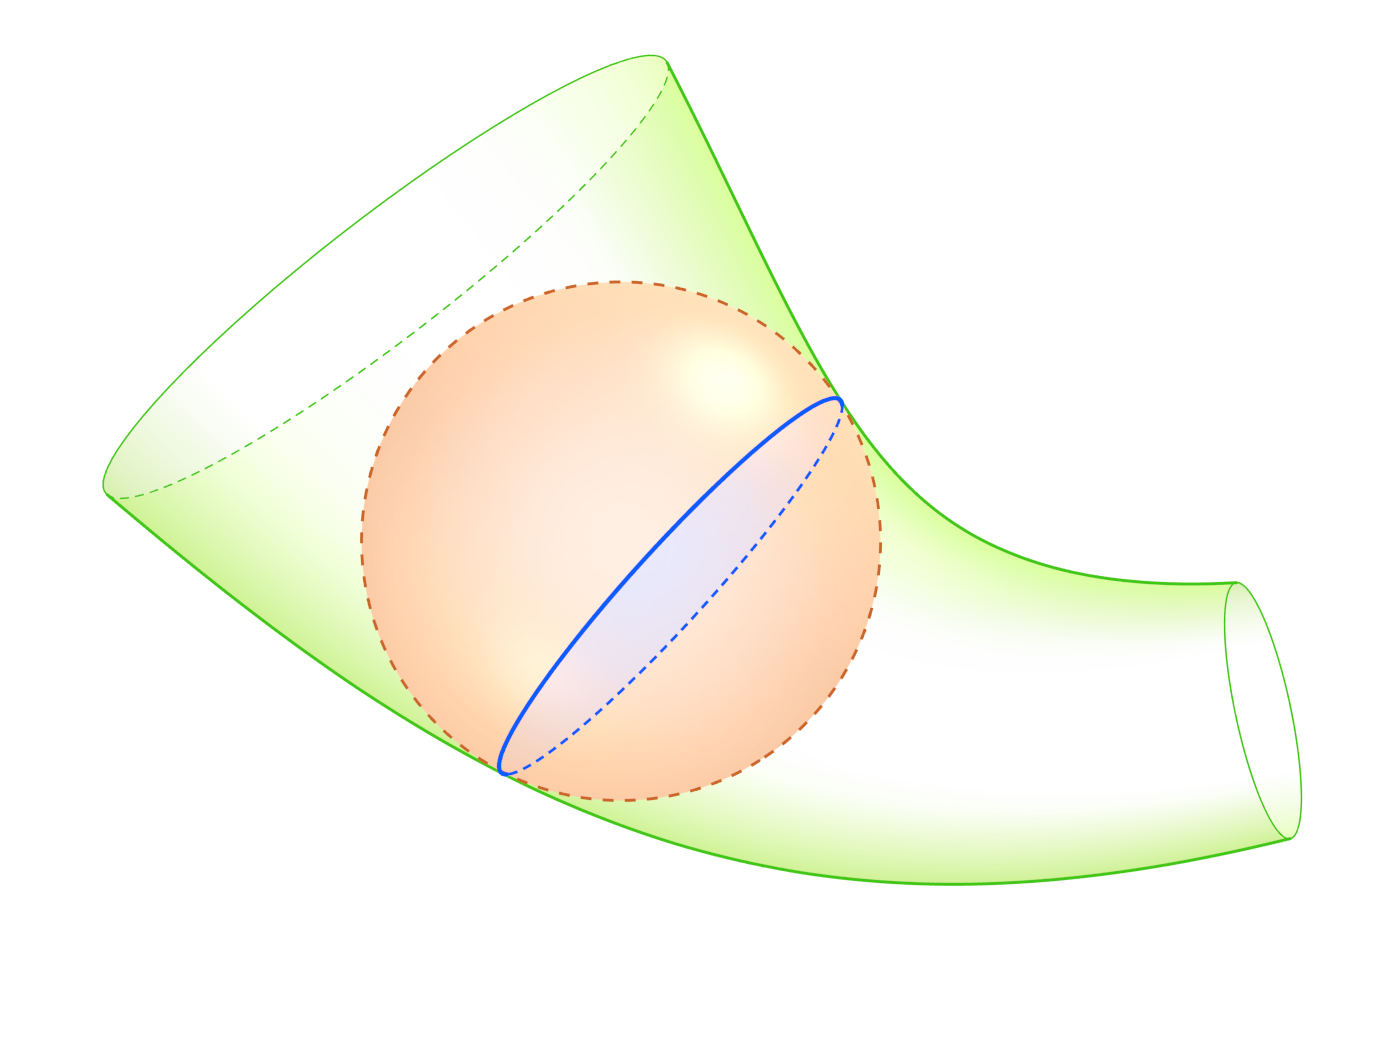
\includegraphics[width=\imagewidth]{figures/images/EdS_propre_courbe/Image0001.png}};
			%
			%\drawGrid{10}{10}{red, thin, dotted}
			%
			\draw[thick, line cap=round] plot file {figures/data/EdS_propre_courbe/spine_xy.dat} node [above right] {$\Gamma$};
			%
			\DTLassign{dbspinepttng}{1}{\gx=x, \gy=y}%
			\coordinate (g) at (\gx, \gy);
			\DTLassign{dbspinepttng}{2}{\dgx=x, \dgy=y}%
			\coordinate (dg) at (\dgx, \dgy);
			\draw[vector] (g) -- (dg) node[txt, below] {$\bg'(u)$};
			\node[txt, left] at (g) {$\bg(u)$};
			\node[point] at (g) {};
			%
			\DTLassign{dbcirclectrpt}{1}{\occx=x, \occy=y}%
			\coordinate (occ) at (\occx, \occy);
			\node[txt, below left, inner sep=0, colorCercle, shift={(1pt,-1pt)}] at (occ) {$\bo(u)$};
			%
			\DTLassign{dbenvelope}{1}{\edsx=x, \edsy=y}%
			\node[colorEdS, above] at (\edsx, \edsy) {$\EdSpropre{\Gamma}{\rho}$};
			%
			\DTLassign{dbenvelope}{2}{\ex=x, \ey=y}%
			\coordinate (e) at (\ex, \ey);
			\node[txt, left, colorEdSPoint] at (e) {$\eos(u,v)$};
			%\draw [dotted, thick, <-, ->] (occ) -- node[txt, right] {$r(u)$} (e);
			\draw [dotted, thick] (occ) -- (e);
			\node[point, fill=colorCercle] at (occ) {};
			%
			\DTLassign{dbenvelope}{3}{\rx=x, \ry=y}%
			\coordinate (r) at (\rx, \ry);
			\draw[vector] (e) -- (r) node[txt, right] {$\br(u,v)$};
			\node[point, colorEdSPoint] at (e) {};
			\node[colorSphere] at (0.31,0.55) {$\sphere[u]$};
			%
			\DTLassign{dbenvelope}{4}{\cx=x, \cy=y}%
			\coordinate (c) at (\cx, \cy);
			\node[txt, left, colorCercle] at (c) {$\circlenotation(u)$};
		\end{scope}
		%
		%\draw[red, dotted, thin] (current bounding box.south west) rectangle (current bounding box.north east);
	\end{tikzpicture}
	\DTLgdeletedb{dbspinepttng}%
	\DTLgdeletedb{dbcirclectrpt}%
	\DTLgdeletedb{dbenvelope}%
	\caption{Paramétrisation de l'EdS propre d'un arc paramétrique.}%
	\label{fig:parametrisation_EdS_propre_courbe}%
\end{figure}